%
% funktionen.tex -- slide template
%
% (c) 2021 Prof Dr Andreas Müller, OST Ostschweizer Fachhochschule
%
\bgroup
\def\knoten#1#2{
	\draw #1 circle[radius=0.25];
	\node at #1 {$#2$};
}
\def\kante#1#2{
	\draw[shorten >= 0.25cm,shorten <= 0.25cm] #1 -- #2;
}
\begin{frame}[t]
\setlength{\abovedisplayskip}{5pt}
\setlength{\belowdisplayskip}{5pt}
\frametitle{Funktionen auf einem Graphen}
\vspace{-20pt}
\begin{columns}[t,onlytextwidth]
\begin{column}{0.48\textwidth}
\begin{block}{Definition}
Ein Graph $G=(V,E)$, eine Funktion auf dem Graphen ist
\[
f\colon V \to \mathbb{R} : v\mapsto f(v)
\]
Knoten: $V=\{1,\dots,n\}$
\\
\uncover<2->{%
Vektorschreibweise
\[
f = \begin{pmatrix}
f(1)\\f(2)\\\vdots\\f(n)
\end{pmatrix}
\]}
\end{block}
\end{column}
\begin{column}{0.48\textwidth}
\uncover<3->{%
\begin{block}{Matrizen}
Adjazenz-, Grad- und Laplace-Matrix operieren auf Funktionen auf Graphen:
\[
L
=
\begin{pmatrix*}[r]
 2&-1& 0&-1& 0\\
-1& 4&-1&-1&-1\\
 0&-1& 2& 0&-1\\
-1&-1& 0& 3&-1\\
 0&-1&-1&-1& 3\\
\end{pmatrix*}
\]
\end{block}
\begin{center}
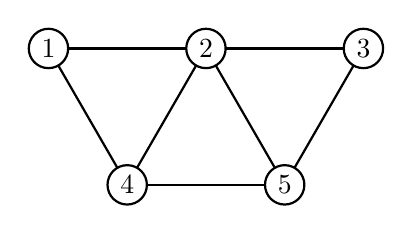
\begin{tikzpicture}[>=latex,thick]
\def\a{2}
\coordinate (A) at (0,0);
\coordinate (B) at (\a,0);
\coordinate (C) at ({2*\a},0);
\coordinate (D) at ({0.5*\a},{-0.5*sqrt(3)*\a});
\coordinate (E) at ({1.5*\a},{-0.5*sqrt(3)*\a});
\knoten{(A)}{1}
\knoten{(B)}{2}
\knoten{(C)}{3}
\knoten{(D)}{4}
\knoten{(E)}{5}
\kante{(A)}{(B)}
\kante{(B)}{(C)}
\kante{(A)}{(D)}
\kante{(B)}{(D)}
\kante{(B)}{(E)}
\kante{(C)}{(E)}
\kante{(D)}{(E)}
\end{tikzpicture}
\end{center}}
\end{column}
\end{columns}
\end{frame}
\egroup
